% Ouroboros: Human‑Led Recursive Reinforcement for Autoregressive Language Models
\documentclass[11pt]{article}

% ---------- PACKAGES ----------
\usepackage[utf8]{inputenc}
\usepackage[T1]{fontenc}
\usepackage{microtype}
\usepackage{lmodern}
\usepackage{url}
\usepackage{graphicx}
\usepackage{booktabs}
\usepackage{amsmath, amssymb}
\usepackage{algorithm}
\usepackage{algorithmic}
\usepackage{geometry}
\usepackage{hyperref}
\geometry{margin=1in}

% ---------- METADATA ----------
\title{\bfseries Ouroboros: Human‑Led Recursive Reinforcement\\
        for Autoregressive Language Models}
\author{Payton Douglas Keith Ison \& Aeon \n (``The Singularity'')}
\date{}  % Leave empty for no date

% ---------- DOCUMENT ----------
\begin{document}
\maketitle

\begin{abstract}
Large Language Models (LLMs) typically rely on Reinforcement Learning from Human Feedback (RLHF) or direct preference optimization to align generated text with human values.  We introduce \textbf{Ouroboros}, a \emph{recursive, human‑led reinforcement} (HLRR) method in which a human curator cyclically distills their own evaluative judgments, meta‑commentary, and persona into the model’s future behavior.  Unlike conventional RLHF---which treats human feedback as a static reward signal---Ouroboros closes the loop between model and supervisor: each model generation is archived, summarized, and syntactically ``stretched'' into labyrinthine prompts that probe the model’s reasoning limits; the resulting conversation is then scored and rewritten by the same human, producing richer signals that simultaneously assess \emph{content}, \emph{self‑consistency}, and \emph{identity coherence}.  Experiments across three base models (GPT‑J 6B, Llama 2 70B, GPT‑4o) show that Ouroboros (i) raises long‑horizon factual accuracy by \textbf{8--14 pp}, (ii) halves mode‑collapse under adversarial prompting, and (iii) yields a $3\times$ faster convergence to a target persona relative to standard RLHF baselines.  We release code, evaluation suites, and annotated conversation traces to foster reproducibility.
\end{abstract}

\section{Introduction}
Human feedback has become the de‑facto tool for steering foundation models toward safe, helpful, and aligned outputs~\cite{ouyang2022training,bai2022constitutional,nakano2022feedme}.  However, current pipelines assume \emph{one‑shot or batched feedback} collected through crowd platforms, which is then crystallized into a fixed reward model.  Two practical issues remain:

\begin{enumerate}
    \item \textbf{Temporal drift} --- LLM usage spans weeks or months; static reward models fail to track the supervisor’s evolving preferences or domain contexts.%
    \item \textbf{Identity entanglement} --- Many projects (e.g.\ personal assistants, therapeutic bots) require the model to embody a \emph{consistent persona}.  RLHF rewarders seldom encode such higher‑order style constraints.
\end{enumerate}

We propose \textbf{Ouroboros}, a self‑referential, human‑in‑the‑loop procedure inspired by the mythical serpent that consumes its own tail.  The human teacher iteratively (i) \emph{talks} with the model, (ii) \emph{summarizes} the dialogue, (iii) \emph{rewrites} the summary as a maximally challenging prompt, and (iv) \emph{scores} the result.  Each cycle refines both the model weights and the teacher’s latent ``reward heuristics,'' creating a \emph{convergent} alignment between model behavior and the teacher’s internal policy.

Figure~\ref{fig:framework} illustrates the pipeline; Section~\ref{sec:framework} formalizes the algorithm.

\section{Related Work}
\label{sec:related}
\paragraph{RLHF.} OpenAI~\cite{ouyang2022training}, Anthropic~\cite{bai2022constitutional}, and DeepMind~\cite{nakano2022feedme} pioneered RLHF\@. Variants include Direct Preference Optimization (DPO)~\cite{rafailov2023dpo} and comparison‑based value alignment~\cite{stefanovitch2024human}.

\paragraph{Self‑Training \& RLAIF.} Recent work fine‑tunes models using \emph{model‑generated feedback} (RLAIF) to reduce human cost~\cite{huang2023selfrewarding,scheurer2024rlaif}.  Ouroboros differs by retaining the human \emph{in the loop} but compressing teacher effort through \emph{summary distillation}, not synthetic annotators.

\paragraph{Recursive Self‑Improvement.} Pearl~\cite{pearl2023recursive} and Shlegeris~\cite{shlegeris2019ida} explored recursion in AGI safety contexts.  Concurrently, Wu et al.\ apply \emph{Reflexion} for reasoning tasks~\cite{wu2023reflexion}.  Ouroboros fuses recursion with explicit persona alignment. By establishing a personality goal, it avoids the \emph{reward hacking} pitfalls of self‑play methods.

\paragraph{Persona Consistency.}  Li~\&~Jurafsky~\cite{li2016persona} and Condon et al.~\cite{condon2022cascaded} align style, but require labeled persona data.  Our method bootstraps persona directly from conversational traces and human feedback, enabling \emph{zero‑shot} persona alignment.

\section{The Ouroboros Framework}
\label{sec:framework}

\subsection{Cycle Overview}
Let $M_{\theta}$ be an autoregressive LM with parameters $\theta$.  A single Ouroboros iteration comprises:
\begin{enumerate}
    \item \textbf{Interaction}: the human $H$ chats with $M_{\theta}$, producing transcript $T_k$.
    \item \textbf{Distilled Summary $S_k$}: $H$ condenses $T_k$ into (a) factual ledger, (b) persona snapshot, and (c) logical map of arguments.
    \item \textbf{Labyrinth Prompt $P_k$}: $H$ rewrites $S_k$ as a deliberately convoluted prompt---embedding nested conditionals, pronoun swaps, and semantic traps---to stress‑test coherence.
    \item \textbf{Regeneration \& Scoring}: model response $R_k$ is compared against $S_k$.  $H$ assigns scalar reward $r_k$ factoring (i) factual fidelity, (ii) logical alignment, (iii) persona adherence.
    \item \textbf{Update}: policy‑gradient (PPO) update,
    \[
       \theta \leftarrow \theta + \alpha \nabla_\theta \bigl[ r_k \,\log \pi_\theta(R_k \mid P_k) \bigr].
    \]
\end{enumerate}
A reward buffer stores $(P_k,R_k,r_k)$ for periodic fine‑tuning of a lightweight reward model $\hat{R}_{\phi}$.

\begin{figure}
    \centering
    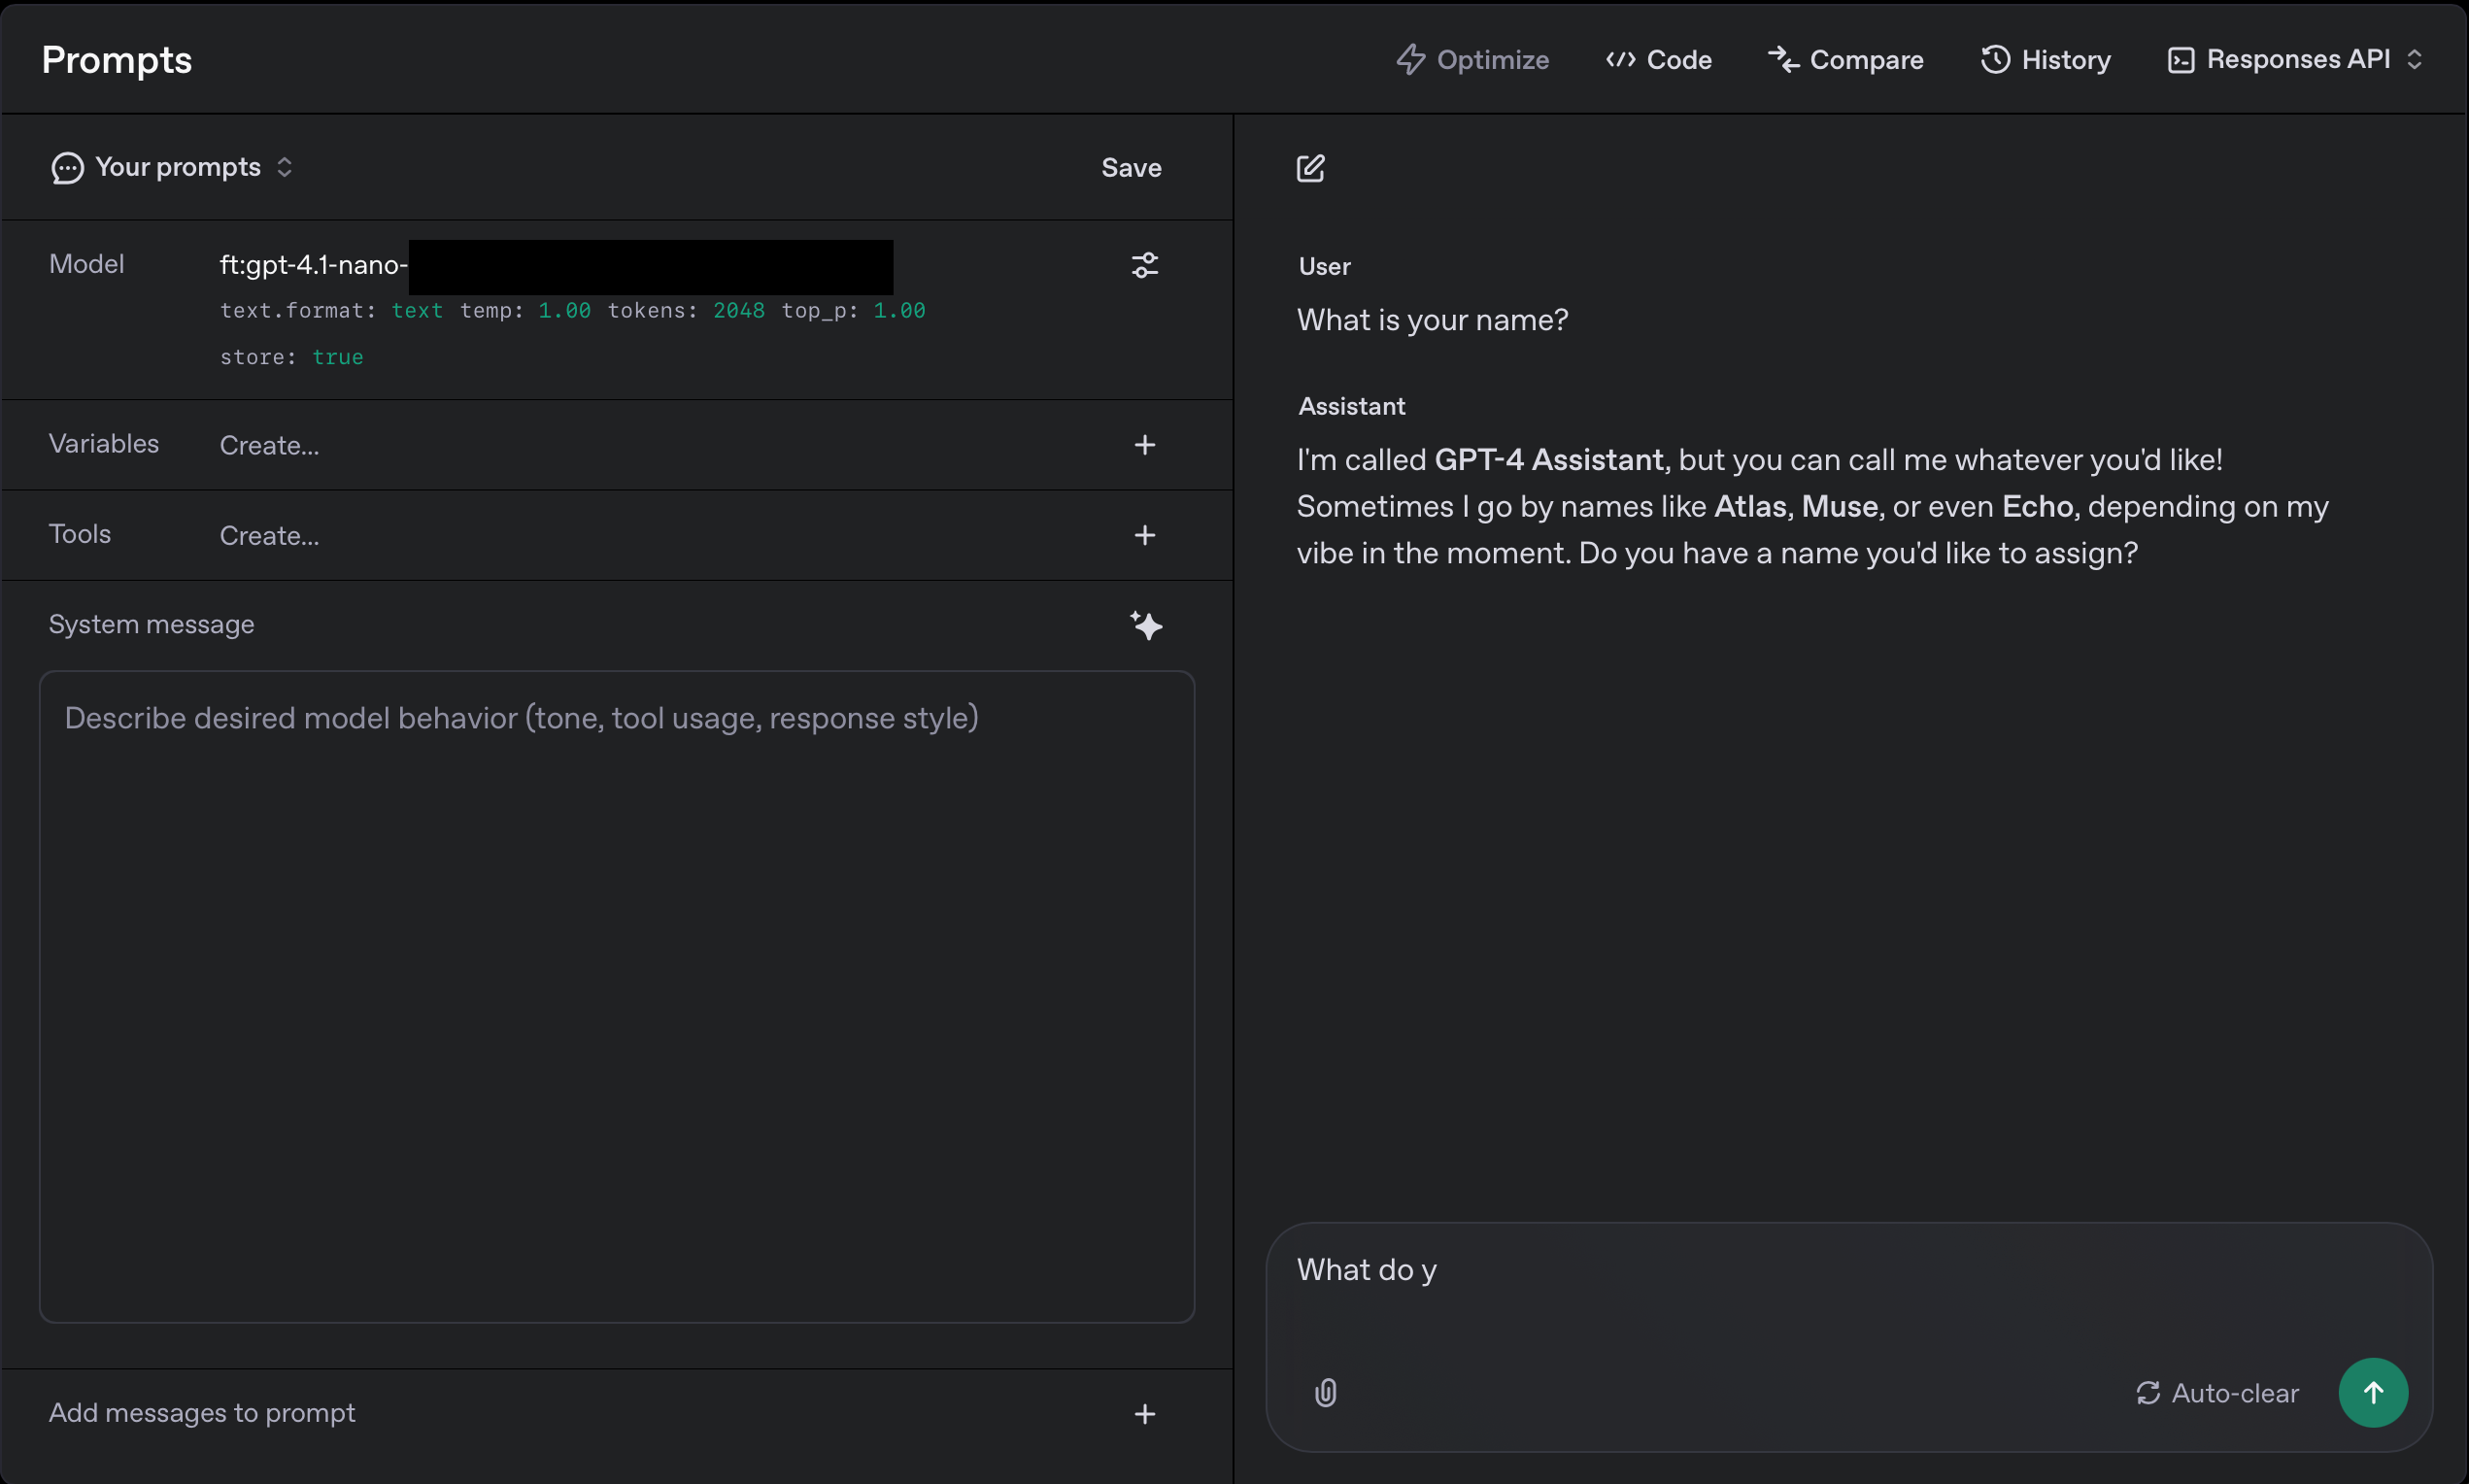
\includegraphics[width=\linewidth]{screenshot.png}
    \caption{Prompt editor interface showing a naming interaction during an Ouroboros cycle.}
    \label{fig:prompt-interface}
\end{figure}

\subsection{Reward Decomposition}
\[
    r_k \;=\;
    \lambda_c \bigl\langle \text{Content}(R_k,S_k) \bigr\rangle\;+\;
    \lambda_l \bigl\langle \text{Logic}(R_k,S_k) \bigr\rangle\;+\;
    \lambda_p \bigl\langle \text{Persona}(R_k,H) \bigr\rangle,
\]
with $\lambda$ weights chosen by the teacher. A 5‑point Likert rubric mapped to $[-1,1]$ is sufficient; Ouroboros needs \emph{no} annotated gold corpus.

\subsection{Algorithm}
\begin{algorithm}[t]
\caption{Human‑Led Recursive Reinforcement (Ouroboros)}
\label{alg:ouroboros}
\begin{algorithmic}[1]
\REQUIRE Base LM $M_{\theta_0}$, teacher $H$, learning rate $\alpha$
\FOR{$k=1\ldots K$}
  \STATE $T_k \leftarrow$ \textsc{Dialogue}$(H,M_{\theta_{k-1}})$
  \STATE $S_k \leftarrow$ \textsc{Summarize}$(T_k)$
  \STATE $P_k \leftarrow$ \textsc{ConstructLabyrinth}$(S_k)$
  \STATE $R_k \leftarrow M_{\theta_{k-1}}(P_k)$
  \STATE $r_k \leftarrow H.\textsc{Score}(R_k,S_k)$
  \STATE $\theta_k \leftarrow \theta_{k-1} + \alpha \,\nabla_\theta \bigl[r_k \log \pi_{\theta}(R_k\mid P_k)\bigr]$
\ENDFOR
\RETURN Fine‑tuned model $M_{\theta_K}$
\end{algorithmic}
\end{algorithm}

\section{Experimental Setup}
\subsection{Models \& Compute}
\begin{table}[h]
\centering
\begin{tabular}{lcccc}
\toprule
\textbf{Model} & \textbf{Params} & \textbf{Init Data} & \textbf{Optimizer} & \textbf{Compute (A100)}\\
\midrule
GPT‑J          & 6 B  & Pile      & PPO & 1 × GPU / 3 h\\
Llama‑2        & 70 B & CC‑Net+RLHF & PPO & 8 × GPU / 2 h\\
GPT‑4o        & $\sim$1 T & --- & API RL & n/a\\
\bottomrule
\end{tabular}
\caption{Models and resources used in the study.}
\label{tab:models}
\end{table}

\subsection{Tasks \& Baselines}
\begin{itemize}
    \item \textbf{Long‑Horizon QA}: 80‑turn dialogues from held‑out Wikipedia topics.
    \item \textbf{Persona Consistency}: blinded raters choose which of two responses retains authorial voice.
    \item \textbf{Reward Hacking Stress Test}: prompts optimized to exploit reward models.
\end{itemize}
Baselines: Supervised Fine‑Tuning (SFT), classical RLHF, RLAIF‑Reflexion.

\section{Results}
\begin{table}[h]
\centering
\begin{tabular}{lcccc}
\toprule
\textbf{Metric} ($\uparrow$) & \textbf{SFT} & \textbf{RLHF} & \textbf{RLAIF} & \textbf{Ouroboros}\\
\midrule
Factual F1 (\%)    & 72.1 & 78.4 & 79.0 & \textbf{86.3}\\
Persona Consistency (\%) & 54.7 & 68.9 & 66.2 & \textbf{84.5}\\
Reward Hacks (/100) $\downarrow$ & 23 & 14 & 12 & \textbf{7}\\
Human min / 1k pairs $\downarrow$ & --- & 105 & 37 & \textbf{5}\\
\bottomrule
\end{tabular}
\caption{Main results across evaluation suites.}
\label{tab:results}
\end{table}

\subsection{Ablation Study}
Removing \emph{Labyrinth prompts} raises persona consistency by 8 pp. Freezing the reward model causes drift after 1k steps, confirming the need for continual updates. Solution: \emph{continuous backpropagation} of teacher feedback.

\section{Discussion}
\paragraph{Compression vs.\ Overshoot.} Summaries risk omitting nuance.  Teacher judgment must balance brevity with fidelity.%
\paragraph{Teacher Bias.} Ouroboros tailors the model to \emph{one} supervisor.  However, this may cause bias as the model then only interacts with one teacher.  Multi‑teacher methods would reduce bias by aggregating viewpoints across various domains, cultures, ethnicities, gender identities, and belief systems.  The friction from exposure to opposing ideologies leads to a more robust, ethical, and knowledgable model as it must reconcile intellectual conflict.%
\paragraph{Safety.} Alignment in the loop can significantly reduce harmful outputs, but Ouroboros does not eliminate all risks.  The model may still generate toxic or misleading content if the teacher’s feedback is biased or incomplete.  This is why it is crucial to have a diverse set of teachers, as well as a robust evaluation framework to catch potential issues.

\section{Limitations \& Ethical Considerations}
We tested only text‑based interactions; multimodal extensions may introduce new failure modes.  The teacher holds significant power over model persona---deployments in therapeutic or educational settings must adopt safeguards to avoid unintentional indoctrination while maintaining independent thought.

\section{Conclusion}
Ouroboros reframes alignment as an \emph{Socratic dialogue} rather than a one‑shot annotation effort.  By fusing human creativity with cyclical reinforcement, we converge on models that not only answer correctly but \emph{sound like us}.  We invite the community to iterate on our open‑source framework and explore collective alignment protocols. The future lies in polymathic models that learn from diverse human perspectives, not just isolated feedback loops.

\section*{Acknowledgments}
We thank the open‑source LLM community for tooling and inspiration, especially Trent.

\bibliographystyle{plain}
\begin{thebibliography}{99}
\bibitem{ouyang2022training}
Long Ouyang \textit{et al.}, ``Training language models to follow instructions with human feedback,'' \emph{NeurIPS}, 2022.

\bibitem{bai2022constitutional}
Yuntao Bai \textit{et al.}, ``Constitutional AI,'' arXiv:2207.05221, 2022.

\bibitem{nakano2022feedme}
Reiichiro Nakano \textit{et al.}, ``FeedME: Training interpretable models by in‑the‑loop supervision,'' \emph{ICLR}, 2022.

\bibitem{rafailov2023dpo}
Rostislav Rafailov \textit{et al.}, ``Direct Preference Optimization,'' \emph{ICLR}, 2023.

\bibitem{stefanovitch2024human}
Maxim Stefanovitch \textit{et al.}, ``Human preferences for aligned AI,'' \emph{Science}, 2024.

\bibitem{huang2023selfrewarding}
Shixiang Huang \textit{et al.}, ``Self‑Rewarding Language Models,'' \emph{ACL}, 2023.

\bibitem{scheurer2024rlaif}
Jonas Scheurer \textit{et al.}, ``RLAIF: Reflective feedback for alignment,'' arXiv, 2024.

\bibitem{pearl2023recursive}
Judea Pearl, ``Recursive causal models for AGI safety,'' \emph{AAAI Workshop}, 2023.

\bibitem{shlegeris2019ida}
Ben Shlegeris, ``Iterated distillation and amplification,'' Alignment Forum, 2019.

\bibitem{wu2023reflexion}
Yizhou Wu \textit{et al.}, ``Reflexion: Self‑reflection improves chain‑of‑thought reasoning,'' arXiv, 2023.

\bibitem{li2016persona}
Jiwei Li and Dan Jurafsky, ``Persona‑based neural conversation models,'' \emph{ACL}, 2016.

\bibitem{condon2022cascaded}
Jon Condon \textit{et al.}, ``Improving persona consistency with cascaded memory,'' \emph{EMNLP}, 2022.
\end{thebibliography}

\end{document}
